\section{Question 11.4}

\subsection{Question}
Show how the linear feature-based ranking function is related to the abstract ranking model from Chapter 5.


\subsection{Answer}
Starting with the first mention of the abstract ranking model, refer to Figure \ref{fig:51}.  This is an example of the ranking function for a single document.

\begin{figure}[H]
\centering
\label{fig:51}
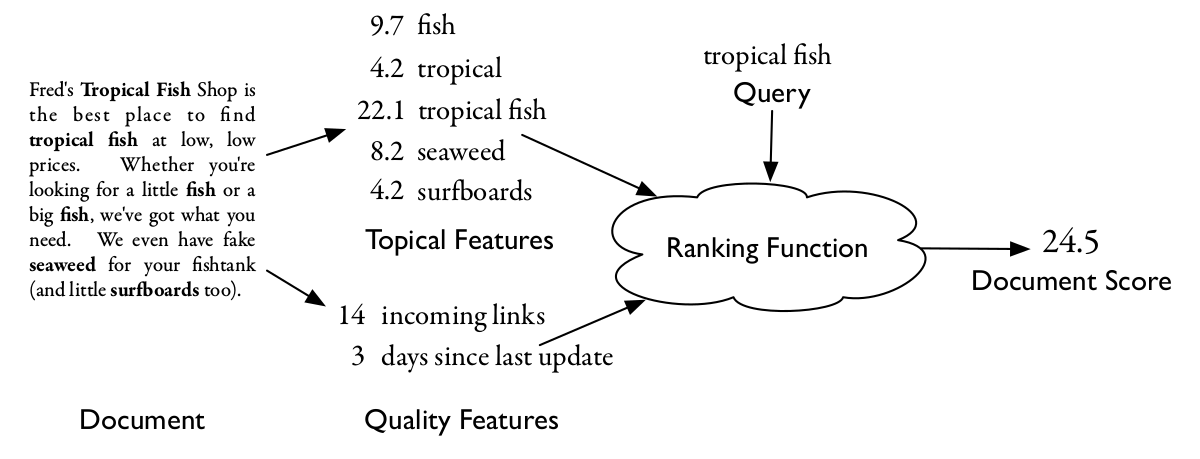
\includegraphics[scale=.25]{q11.4/fig51.png}
\caption{The components of the abstract model of ranking\dots}
\end{figure}

And a more formal definition of the abstract ranking model can be found in equation \ref{eq:1}:

\begin{equation}
\label{eq:1}
R(Q, D) = \sum_i g_i (Q) f_i (D)
\end{equation}

This is a linear combination of two feature functions, \(f_i\) is a feature function that extracts a score from the document and \(g_i\) is a feature function that extracts a score from the query.\\

Now, for a definition of the linear feature-based retrieval model, refer to Equation \ref{eq:2}:

\begin{equation}
\label{eq:2}
S_\Lambda(D;Q) = \sum_j \lambda_j \cdot f_j(D, Q) + Z
\end{equation}

here, \(f_j\) is a feature function that maps query/document pairs to real values, i.e. scores, so it is also a linear combination of functions that emit scores based on features of some related piece of the components of the formulation, either the document, the query, some parameter (\(\lambda \in \Lambda\)), or a constant that is not related to the document but could be related to the query (\(Z\)).  This is very similar to how the abstract ranking model functions in that it is a summation of a group of scoring functions over the elements to be ranked.  The mechanism is the same as before with the abstract model, with the addition of the \(\lambda\) parameters.
